% Paper 1 -- the phase-trap letter. Every number carries its RESULTS.md row id in a
% LaTeX comment; do not edit numbers here without the ledger. Build:
%   pdflatex main.tex && pdflatex main.tex
\documentclass[a4paper,11pt]{quantumarticle}
\pdfoutput=1
\usepackage[utf8]{inputenc}
\usepackage[T1]{fontenc}
\usepackage{amsmath,amssymb}
\usepackage{graphicx}
\usepackage{booktabs}
\usepackage{hyperref}

\newcommand{\chiAB}{\chi_{AB}}

\begin{document}

\title{A phase trap in approximate circuit compilation: how a converged compiler silently breaks interferometric protocols, and a one-gate fix}

% TODO(team): author order, affiliations, and emails are placeholders -- decide before
% submission. All five hackathon members listed alphabetically for now.
\author{Chao Hsien}
\author{Jiwan Kang}
\author{Ng Siu Hin}
\author{Su Wei-Chang}
\author{Tina Tien}
\affiliation{Qiskit Hackathon 2026, Team 8 --- affiliation TBD}



\maketitle

\begin{abstract}
Tensor-network circuit compilation (AQC) can dramatically compress the controlled time
evolution at the heart of a Hadamard test: on an open XXZ chain we measure a crossover
against exact controlled-unitary synthesis at $n=4$ system qubits, growing to a
$36\times$ two-qubit-gate reduction at $n=7$ and $1514\times$ at $n=10$, at state
infidelity below $3\times10^{-4}$ throughout.
% R046, R056
We then show that shipping this compression naively destroys the experiment it was built
for, with no warning from the compiler: the optimisation objective (state fidelity) is
blind to global phase, while a Hadamard test is precisely an interferometer that measures
that phase. A compression that converges to state infidelity $3\times10^{-4}$ returns an
interference signal $\chi$ wrong by $1.22$--$1.35$ on a quantity bounded by
$|\chi|\leq1$.
% R046
The repair costs one single-qubit gate: the offending phase is available for free at
compile time, and a $P(-\theta)$ on the ancilla cancels it exactly, reducing the error to
below $0.01$.
% R046
We delimit the hazard precisely: direct observable estimation on the compiled state is
provably immune, so the trap is specific to interferometric use.
% R060
We demonstrate the trap directly on a superconducting processor: shipped with and
without the fix in one job, the broken and repaired circuits are indistinguishable to
every magnitude metric, while the compile-time phase offset between them survives
$\approx$186 two-qubit gates of device noise coherently, to within $0.06$--$0.13$ rad
of its predicted value --- and the device is found to add coherent phase errors of its
own, equally invisible to magnitude-based certification.
% R061
Finally, we report a pre-registered test of the compilation advantage at $n=6$ on two
superconducting processors: it does not survive present-day error rates, falling short
of its own prediction by a factor of twelve, and we quantify the effective error rate
at which it becomes measurable.
% R053, R054
\end{abstract}

\section{Introduction}
\label{sec:intro}

The Hadamard test is the elementary interferometric primitive of quantum computation: an
ancilla prepared in superposition controls a unitary $U$ on a system register, and the
ancilla statistics estimate the complex overlap $\chi=\langle\psi|U|\psi\rangle$, whose
phase carries the physics (for $U=e^{-iHt}$, the spectrum). It underlies quantum phase
estimation, Krylov-subspace diagonalisation, and the verification of compiled circuits.
Its practical obstacle is the controlled evolution: synthesising an exact controlled-$U$
for an arbitrary $n$-qubit unitary costs $O(4^{n+1})$ two-qubit gates.

Approximate quantum compiling (AQC)~\cite{madden2022,aqctensor} attacks exactly this
cost: a classical tensor-network optimiser finds a shallow parameterised circuit whose
action on a chosen input state matches the deep target circuit, certified by a state
fidelity. It is natural, then, to compile the evolution inside a Hadamard test.

This paper reports three things. First, the compression works, and keeps working well
past the sizes where the exact construction is hopeless
(Sec.~\ref{sec:crossover}). Second --- our central observation --- the compiler's own
success criterion silently breaks the interferometer it is being compiled for
(Sec.~\ref{sec:trap}): state fidelity is a magnitude, a Hadamard test measures a phase,
and the gap between those two sentences is an error as large as the signal, invisible to
every certificate the compilation stack reports. The fix costs one single-qubit gate. We
delimit the hazard by proving --- and verifying on the same compiled circuits --- that
direct observable estimation on the compiled state is immune, so ordinary
(non-interferometric) uses of AQC are unaffected (Sec.~\ref{sec:scope}). Third, the
trap and its fix are demonstrated on a real device, with pre-registered predictions
(Sec.~\ref{sec:trapHW}), and we report a pre-registered falsification of the
compilation advantage itself at $n=6$ on two processors, including a further
independent appearance of the magnitude-hides-phase failure in the hardware data
(Sec.~\ref{sec:hardware}).

The instrument we use to detect and quantify the trap is itself of independent interest:
an \emph{anti-controlled} Hadamard test that interferes two dynamics --- the compiled
circuit $W$ and its target $U$ --- on one ancilla, measuring
$\chiAB(t)=\langle\psi|W^\dagger U|\psi\rangle$ directly on the device
(Sec.~\ref{sec:instrument}). The construction follows the appendices of
Ref.~\cite{faehrmann2025}, whose ``shadow-enhanced'' Hadamard test this project
implements end to end; measuring the otherwise-discarded system register in random bases
\`a la classical shadows~\cite{huang2020} upgrades the scalar verdict to a
per-observable one.

Throughout, the benchmark family is deliberately small (2--10 qubits) and exactly
solvable, so that every estimate is graded against exact truth; we claim no advantage
over classical computation anywhere in this paper. Every number reported here is
reproducible from a public repository whose results ledger records the producing command
for each value.
% House rule: numbers below carry their ledger row ids as comments.

\section{The instrument: an anti-controlled Hadamard test}
\label{sec:instrument}

\begin{figure}[t]
  \centering
  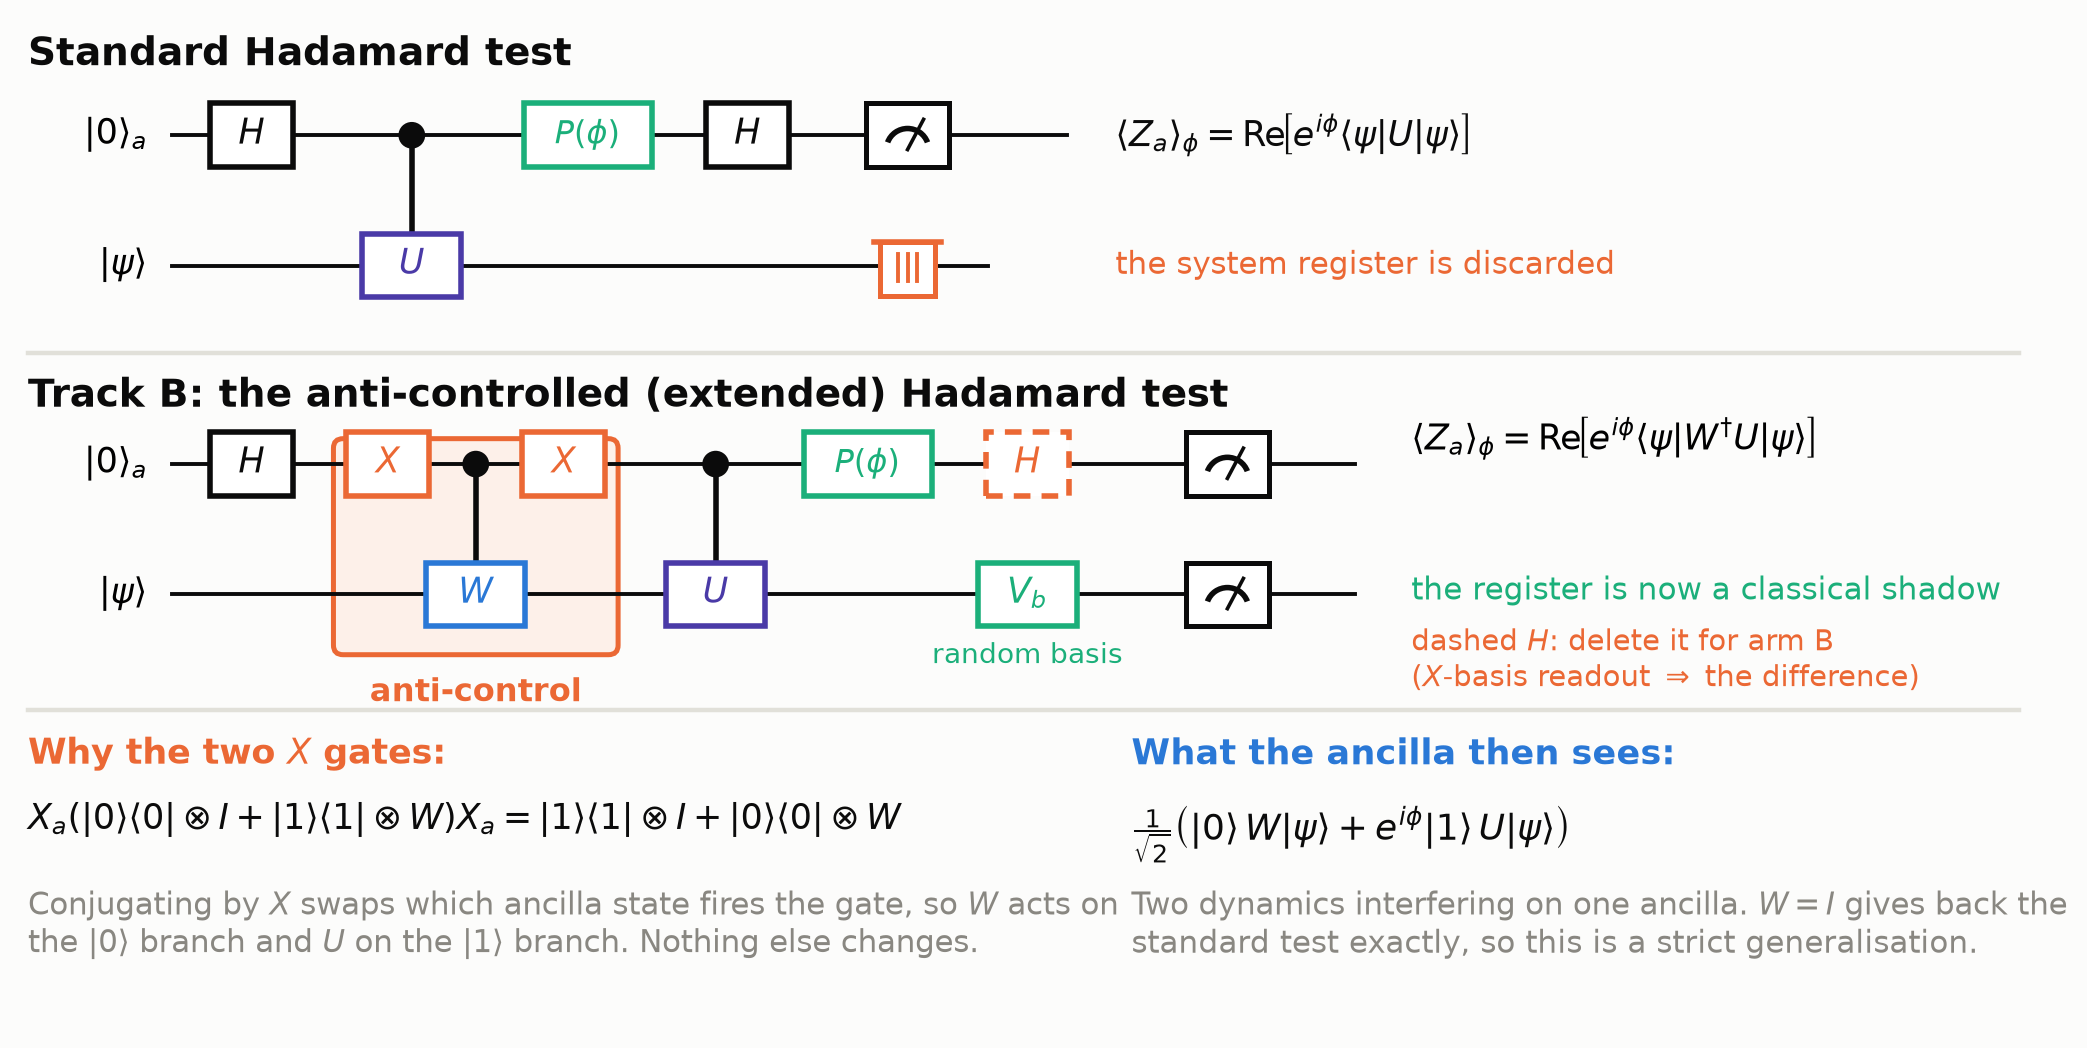
\includegraphics[width=\linewidth]{fig_tb_anticontrol.png}
  \caption{The anti-controlled Hadamard test. Conjugating the controlled-$W$ by $X$ on
  the ancilla makes $W$ fire on the $|0\rangle$ branch while the ordinary controlled-$U$
  fires on the $|1\rangle$ branch, so the ancilla interferes two dynamics:
  $\langle Z_a\rangle_\varphi = \mathrm{Re}\,[e^{i\varphi}\chiAB(t)]$ with
  $\chiAB(t)=\langle\psi|W^\dagger U|\psi\rangle$. Setting $W=I$ recovers the standard
  test. Construction after Ref.~\cite{faehrmann2025}, Apps.~B and E.}
  \label{fig:anticontrol}
\end{figure}

Let $U=e^{-iHt}$ be the target evolution and $W$ any cheaper stand-in --- a Trotter
product formula or a compiled circuit. Sandwiching a controlled-$W$ between two $X$
gates on the ancilla makes $W$ act on the $|0\rangle$ branch; an ordinary controlled-$U$
then acts on the $|1\rangle$ branch (Fig.~\ref{fig:anticontrol}). The ancilla
expectation values in the two quadratures $\varphi\in\{0,-\pi/2\}$ yield the complex
overlap of the two dynamics,
\begin{equation}
  \chiAB(t)=\langle\psi|W^\dagger(t)\,U(t)|\psi\rangle,
  \label{eq:chiAB}
\end{equation}
measured on the device rather than simulated. This is the on-device answer to the
question every practical simulation raises: \emph{how wrong is the circuit you can
afford, relative to the one you meant to run --- and wrong in what?}

Because the circuit is new, it gets its own validation rather than inherited trust: on
our benchmark models the statevector identity between Eq.~\eqref{eq:chiAB} and the
constructed circuit holds to $9.0\times10^{-15}$ ($n=3$) and $4.6\times10^{-15}$
($n=2$).
% R034, R042
Deleting the final Hadamard and measuring the system register in uniformly random Pauli
bases (a classical shadow~\cite{huang2020}) splits the ancilla-tagged records into
estimators of $(W\rho W^\dagger \pm U\rho U^\dagger)/2$, giving every system observable
under $W$ and under $U$ \emph{separately} from the same shots --- a per-observable
disagreement profile on top of the scalar $\chiAB$~\cite{faehrmann2025}.
% R042
We note for completeness that for the scalar overlap alone this instrument is not the
cheapest option: a Loschmidt echo is $4$--$6\times$ cheaper at every size we measured
and, on hardware, substantially more accurate; the anti-controlled test earns its keep
through the phase and the per-observable profile, which no magnitude-only test returns.
% R043, R044

\section{Compilation makes the test scale}
\label{sec:crossover}

\begin{figure*}[t]
  \centering
  
\includegraphics[width=0.92\textwidth]{fig_aqc_scaling.png}
  \caption{Two-qubit gate cost of the controlled evolution on an open XXZ chain at
  $t=0.9$, and the phase trap. The exact controlled block grows as $O(4^{n+1})$; the
  compiled (AQC) circuit grows roughly linearly, with a measured crossover at $n=4$. The
  trap panel shows the compiled circuit's interference error before and after the
  one-gate phase correction of Sec.~\ref{sec:trap}.}
  \label{fig:scaling}
\end{figure*}

The benchmark family is an open XXZ chain,
$H=\sum_{i}[J(X_iX_{i+1}+Y_iY_{i+1})+\Delta Z_iZ_{i+1}]+\sum_i h_i Z_i$ with $J=0.65$,
$\Delta=0.25$ and fixed local fields, evolved to $t=0.9$; the input state is a product
state with a single $R_y(1.3)$ rotation. The honest baseline is the direct synthesis of
$|0\rangle\!\langle0|\otimes I+|1\rangle\!\langle1|\otimes U$ as a single
$(n{+}1)$-qubit unitary --- markedly cheaper than controlling a synthesised circuit, and
therefore harder to beat.
% R046 (baseline note)

Compiling the evolution with the MPS-backed AQC optimiser~\cite{aqctensor,gray2018} and
then controlling the resulting ansatz gives the two-qubit gate counts of
Table~\ref{tab:scaling}. The crossover sits at $n=4$; by $n=7$ the compiled construction
is $35.9\times$ cheaper, by $n=10$, $1514\times$ --- while the compiler's state
infidelity stays flat at $(1.4$--$3.0)\times10^{-4}$ and the (phase-corrected)
interference error stays at $0.008$--$0.010$.
% R046, R056

\begin{table}[b]
  \centering
  \caption{Controlled-evolution two-qubit gate counts (ideal basis-gate counts, no
  routing) and the compiled circuit's error measures. State infidelity is the compiler's
  own certificate; $|\Delta\chi|$ is the interference error after the one-gate phase
  correction of Sec.~\ref{sec:trap}.}
  \label{tab:scaling}
  \begin{tabular}{rrrrcc}
    \toprule
    $n$ & exact & AQC & ratio & state infid. & $|\Delta\chi|$ (fixed)\\
    \midrule
    3  & 50        & 132 & $0.38\times$ & $1.4\times10^{-4}$ & 0.0100\\
    4  & 236       & 216 & $1.09\times$ & $2.6\times10^{-4}$ & 0.0080\\
    5  & 1\,004    & 300 & $3.35\times$ & $2.7\times10^{-4}$ & 0.0082\\
    6  & 4\,140    & 384 & $10.8\times$ & $3.0\times10^{-4}$ & 0.0079\\
    7  & 16\,812   & 468 & $35.9\times$ & $2.9\times10^{-4}$ & 0.0083\\
    8  & 67\,756   & 552 & $122.8\times$ & $2.9\times10^{-4}$ & 0.0083\\
    9  & 272\,044  & 636 & $427.7\times$ & $2.9\times10^{-4}$ & 0.0083\\
    10 & 1\,090\,220 & 720 & $1514\times$ & $2.8\times10^{-4}$ & 0.0082\\
    \bottomrule
  \end{tabular}
  % R046 (n=3..7), R056 (n=8..10)
\end{table}

The advantage is not an artefact of the 1D chain or of idealised connectivity. On a 2D
lattice the crossover shifts by one qubit and the advantage reaches $100.8\times$ at
$n=8$;
% R049
on a $2\times2$ Fermi--Hubbard grid (8 qubits, Jordan--Wigner) the gate advantage is
$34.7\times$, though there the compression accuracy degrades by roughly $30\times$ and
we do not claim it usable without further optimisation;
% R051
and re-transpiling every circuit against a real heavy-hex coupling map \emph{widens} the
advantage in every case measured (e.g.\ $10.8\times\to15.4\times$ at $n=6$), because the
dense exact block pays about $2.1\times$ for routing while the shallow local ansatz pays
about $1.5\times$.
% R052

One scope statement belongs in the main text rather than a footnote: the compiled $W$ is
optimised for \emph{one} input state, and its process infidelity is accordingly large
($\sim0.96$ at $n\geq5$). That is legitimate for a Hadamard test, whose controlled gate
only ever acts on that prepared state, and illegitimate the moment anything feeds the
compiled gate a different input.
% R046

\section{The trap: a phase-blind objective breaks a phase interferometer}
\label{sec:trap}

The AQC objective maximises the state fidelity
$|\langle\psi_{\rm target}|\psi_{\rm ansatz}\rangle|$ --- a magnitude, invariant under
$|\psi_{\rm ansatz}\rangle\to e^{i\theta}|\psi_{\rm ansatz}\rangle$. A Hadamard test
measures precisely that phase. Concretely, a compression that converges to state
infidelity $3\times10^{-4}$ returns
\begin{equation}
  W|\psi\rangle = e^{i\theta}\,U|\psi\rangle,\qquad \theta\ \text{up to}\ 3.0\
  \text{rad},
\end{equation}
and the measured interference signal comes out wrong by
$|\Delta\chi|=1.22$--$1.35$ across $n=3$--$7$ --- on a quantity bounded by
$|\chi|\leq1$, an error as large as the signal itself. No certificate the compilation
stack reports can see it: the objective, the reported infidelity, and the common
``survival'' summary $|\chi_{\rm meas}|/|\chi_{\rm exact}|$ are all magnitudes.
% R046

We nearly missed it ourselves. Our first certification of the compiled circuit used
$|\chiAB|$ --- also a magnitude --- and passed. Only the phase-sensitive readout of the
anti-controlled test (Sec.~\ref{sec:instrument}) exposed the error, which is the
practical argument for phase-sensitive verification of compiled circuits in general.
% R035, R046

\emph{The fix costs one single-qubit gate.} If $W|\psi\rangle=e^{i\theta}U|\psi\rangle$,
then $\theta=\arg\langle U\psi|W\psi\rangle$ is available at compile time --- the same
MPS contraction that certifies the compression evaluates it at negligible extra cost ---
and a phase gate $P(-\theta)$ on the \emph{ancilla} cancels it exactly, because the
ancilla branch carrying $W$ is the one the phase multiplies. The interference error
drops from $1.33$ to $0.008$ at $n=6$, a $135$--$168\times$ improvement across the
range, and the correction is included in every ``fixed'' number of
Table~\ref{tab:scaling}.
% R046

The same magnitude-hides-phase failure appeared twice more, independently. Re-analysing
a hardware dataset taken by teammates on a square-lattice device, one run's survival
read $0.988$ --- near perfect --- while the complex $\chi$ was $22.6\sigma$ from the
exact value, a $0.77$-rad phase error; the magnitude survived the device, the phase did
not.
% R053, R031
The third instance appears in our own hardware experiment below
(Sec.~\ref{sec:hardware}), where a magnitude-only metric crowns a completely dead
circuit the best performer.

\section{Scope of the trap: pure compilation is immune}
\label{sec:scope}

It is important not to overclaim: the trap is \emph{not} a defect of approximate
compilation itself. In its textbook use --- compress a state-preparation circuit, then
measure observables directly on the prepared state --- AQC is provably unaffected,
because an observable expectation value is exactly invariant under the offending phase:
\begin{equation}
  \langle O\rangle_W=\langle\psi|W^\dagger OW|\psi\rangle
  =\langle\psi|U^\dagger e^{-i\theta}Oe^{i\theta}U|\psi\rangle
  =\langle O\rangle_U ,
\end{equation}
for any Hermitian $O$ and any $\theta$. The overlap
$\chi=\langle\psi|U|\psi\rangle$, by contrast, is an interference term between two
states, not an expectation value in any single state, and extracting it physically
requires an ancilla-based circuit --- which is exactly where the phase re-enters.

We verified this on the same compiled circuits as Table~\ref{tab:scaling} (the
interference errors reproduce to four digits, confirming identical compilations): direct
estimation of $\langle Q\rangle$, $\langle H\rangle$ and $\langle Z_0\rangle$ on the
compiled state has worst-case error $0.018$ ($n=3$), $0.014$ ($n=5$) and $0.015$
($n=7$) --- two orders of magnitude below the interferometric error on the same circuit,
and consistent with the compiler's ordinary state infidelity. Multiplying the compiled
state by an arbitrary additional global phase changes every measured observable by less
than $2\times10^{-15}$.
% R060
The trap is therefore specific to embedding compiled circuits inside interferometric
protocols --- Hadamard tests, phase estimation, overlap and echo-type verification ---
and it is exactly there that phase-aware certification, or the one-gate correction
above, is required.

\section{The trap on hardware}
\label{sec:trapHW}

The trap and its fix, as presented so far, live on the statevector. Demonstrating them
on hardware requires a depth at which signal survives, so we ran the standard Hadamard
test at $n=3$ (where the compiled circuit routes to 186 two-qubit gates) with three
arms in \emph{one} job on \texttt{ibm\_marrakesh}: the exact controlled block (101
gates, reference), the compiled ansatz \emph{without} the phase correction, and the
same ansatz \emph{with} it --- identical gate counts, since the correction is a
virtual-$Z$. Three predictions were recorded before submission: (P1) magnitude metrics
cannot separate the broken arm from the repaired one; (P2) the measured phase
difference $\arg(\chi_{\rm naive}/\chi_{\rm fixed})$ equals the compile-time
$\theta(t)$; (P3) the fixed arm's $\chi$ points along the exact $\chi$.
% R061

P1 and P2 were confirmed. The naive/fixed survivals came back statistically
indistinguishable ($0.382/0.390$, $0.349/0.286$, $0.267/0.244$ at $t=0.3,0.6,0.9$),
while the measured inter-arm phases were $-2.235$, $+0.436$, $+2.816$\,rad against
pre-registered $\theta$ values of $-2.179$, $+0.378$, $+2.948$ --- deviations of
$0.06$--$0.13$\,rad. The compiler's phase offset rides \emph{coherently} through
$\approx186$ gates of device noise: fully invisible to every magnitude metric, fully
visible to a phase-sensitive readout.
% R061

P3 was falsified, instructively. The fixed arm does not point along the exact
$\chi$ --- and neither does the \emph{exact} arm, whose survival of $0.86$ coexists
with phase errors of $+0.26$ to $+0.44$\,rad; the deeper compiled arms carry a common
device-induced phase error of $\approx-2.2$\,rad on top of the (exactly cancelled)
compiler phase. The device, like the compiler, contributes coherent phase error that
no magnitude figure of merit can see, and that a compile-time correction cannot
anticipate. We report its cause as unattributed (single run, one device). Both halves
of the experiment therefore compound the paper's thesis: phase errors --- from the
compiler \emph{and} from the device --- demand phase-sensitive certification.
% R061

\section{Pre-registered scaling test at $n=6$, and its honest failure}
\label{sec:hardware}

\begin{figure}[t]
  \centering
  
\includegraphics[width=\linewidth]{fig_aqc_hw.png}
  \caption{Three constructions of the same $n=6$ Hadamard test on
  \texttt{ibm\_marrakesh} (4\,000 shots per circuit, $t\in\{0.3,0.6,0.9\}$), against
  survival predictions recorded before submission. Every arm returned noise; the
  deliberately hopeless 8\,850-gate exact arm reports an \emph{unphysical} survival
  above~1 --- a $T_1$-relaxation floor that a magnitude-only metric scores as the best
  result on the plot. The $y$-axis deliberately extends past $|\chi|=1$ to show it.}
  \label{fig:hw}
\end{figure}

A compilation advantage measured in gate counts is not yet a hardware advantage. We
submitted the same $n=6$ Hadamard test built three ways --- exact controlled block
(8\,850 two-qubit gates after routing), controlled Trotter ($2\,119$), and compiled AQC
with the phase fix ($576$) --- to two superconducting processors, with survival
predictions written down before submission so that failure would be undeniable.
% R054

It was. On \texttt{ibm\_marrakesh} the compiled arm returned mean survival $0.026$
against a predicted $0.315$; on \texttt{ibm\_kingston}, $0.033$ against $0.401$ ---
twelve times short on both devices, statistically indistinguishable from the
$2\,119$-gate Trotter arm, with mean interference errors $\approx0.83$ on a unit-bounded
quantity.
% R054
The exact arm is the most instructive failure: its ``survival'' reads $1.49$
(marrakesh) and $1.19$ (kingston) --- unphysical, since $|\chi|\leq1$. Both quadratures
sit pinned near a constant, which is the ancilla relaxed to $|0\rangle$: at
$8\,850$ gates the circuit runs for $\approx8\,T_2$, and what the metric scores is $T_1$
relaxation, not signal. A magnitude-only figure of merit crowns the deadest circuit the
winner --- the third independent sighting of the pattern of Sec.~\ref{sec:trap}.
% R054

From the measured survivals, the effective error per two-qubit gate is
\emph{bounded below} by $\varepsilon_{\rm eff}\geq-\ln(S)/N_{2q}\approx6\times10^{-3}$
--- a bound rather than an estimate, because the measured $|\chi|$ sits near the
estimator's own counting-noise floor $\sigma\sqrt{\pi/2}\approx0.020$ at these shot
counts.
% R054 (C7 correction), R058
A shot-count sweep ($2\,000/4\,000/8\,000$ shots, same circuits, same device) supports
reading this as a genuine error floor rather than shot-starvation: doubling the shots
from $4\,000$ to $8\,000$ should shrink a pure counting floor by $29\%$, but the
measured survival moved only $7\%$ ($0.026\to0.024$), and the inferred bound stabilises
at $6.3$--$6.4\times10^{-3}$ --- with the caveat that the three shot counts are separate
jobs on different days, so device drift is not excluded.
% R058
Visibility of the compiled signal at this depth requires
$\varepsilon_{\rm eff}\lesssim2\times10^{-3}$: a gap of at least $3\times$, roughly one
device generation, and not something a larger $n$ improves --- transpiling the full
experiment at $n=7$ shows the compilation \emph{ratio} doubling while the absolute
compiled depth grows and the predicted signal halves.
% R054, R055

\section{Discussion}
\label{sec:discussion}

The finding is small to state and broad to apply: \emph{any} pipeline that compiles or
optimises circuits against a magnitude-only objective, and then consumes the result
interferometrically, inherits an uncertified phase degree of freedom that can be as
large as the signal. The instances here --- a tensor-network compiler's objective, a
survival summary statistic, and a relaxation floor on hardware --- are three faces of
one mistake: certifying an interferometer with a magnitude. The cure is equally simple
to state: certify with a phase-sensitive quantity (the anti-controlled test of
Sec.~\ref{sec:instrument} is one such instrument, and for the scalar question a
Loschmidt echo is cheaper), or cancel the phase at compile time, where it is available
for free.

Three honest limitations. First, everything here is measured on one benchmark family at
$2$--$10$ qubits, exactly solvable by design so that every number is graded against
truth; no claim is made beyond it, and none against classical computation. Second, the
compiled circuits are single-input-state compressions; their process infidelity is
large, and every use beyond the Hadamard test they were compiled for is out of scope.
Third, the hardware negative is two single runs per device configuration with
pre-registered predictions, not a device characterisation; the residual factor
$\sim7\times$ between our noise-budgeted prediction and the measured survival is
reported as unattributed rather than explained.
% R054

\section*{Data and code availability}
All circuits, evidence files, and the results ledger that sources every number in this
paper (row identifiers are embedded as comments in the manuscript source) are public at
\url{https://github.com/mnsh0409/Qiskit-Hackathon-2026}.

\section*{Acknowledgments}
% TODO(team): funding, IBM Quantum access acknowledgment wording, hackathon organisers.
This work was carried out as part of the Qiskit Hackathon 2026 (Topic~5). We acknowledge
the use of IBM Quantum services; the views expressed are those of the authors and do not
reflect the official policy of IBM or the IBM Quantum team.

\begin{thebibliography}{9}
% All entries verified 2026-08-16 against the arXiv abstract pages / journal records.
\bibitem{faehrmann2025} P.~K. Faehrmann, J. Eisert, and R. Kueng,
\emph{In the shadow of the Hadamard test: Using the garbage state for good and further
modifications}, Phys. Rev. Lett. \textbf{135}, 150603 (2025); arXiv:2505.15913.

\bibitem{huang2020} H.-Y. Huang, R. Kueng, and J. Preskill,
\emph{Predicting many properties of a quantum system from very few measurements},
Nat. Phys. \textbf{16}, 1050 (2020).

\bibitem{madden2022} L. Madden and A. Simonetto,
\emph{Best approximate quantum compiling problems},
ACM Trans. Quantum Comput. \textbf{3}(2), 7 (2022); arXiv:2106.05649.

\bibitem{aqctensor} \emph{Qiskit addon: approximate quantum compilation with tensor
networks} (\texttt{qiskit-addon-aqc-tensor}), v0.3.1,
\url{https://github.com/Qiskit/qiskit-addon-aqc-tensor}.

\bibitem{gray2018} J. Gray,
\emph{quimb: a python library for quantum information and many-body calculations},
J. Open Source Softw. \textbf{3}(29), 819 (2018).

\bibitem{khatri2019} S. Khatri, R. LaRose, A. Poremba, L. Cincio, A.~T. Sornborger, and
P.~J. Coles, \emph{Quantum-assisted quantum compiling}, Quantum \textbf{3}, 140 (2019).

\bibitem{qiskit} A. Javadi-Abhari \emph{et al.},
\emph{Quantum computing with Qiskit}, arXiv:2405.08810 (2024).
\end{thebibliography}

\end{document}
